\documentclass{article}
\usepackage[utf8]{inputenc}
\usepackage{hyperref}
\usepackage{graphicx}
\usepackage{float}

\title{ECE 4310\\Operating Systems for Embedded Application\\\,\\Project 1}
\author{Choi Tim Antony Yung}
\date{March 4, 2021}
\begin{document}
\maketitle

\thispagestyle{empty}
\setcounter{page}{0}

\newpage

\section{Unix login server}

\subsection{\texttt{ls -l /}}

\begin{figure}[H]

  \caption{Output of \texttt{ls -l /}}
  \centering
  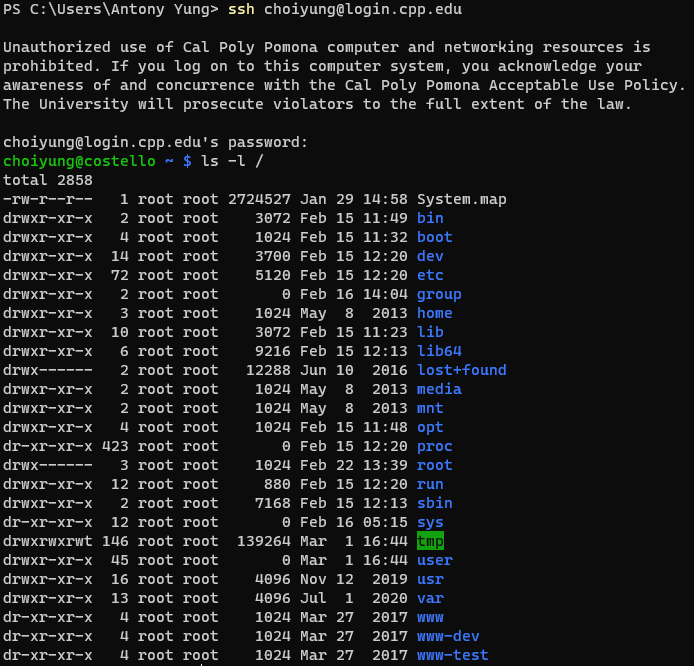
\includegraphics[width=0.75\textwidth]{ECE4310_proj1_part1_1a.png}
\end{figure}

\begin{figure}[H]
  \caption{Output of \texttt{ls -l /lib}}
  \centering
  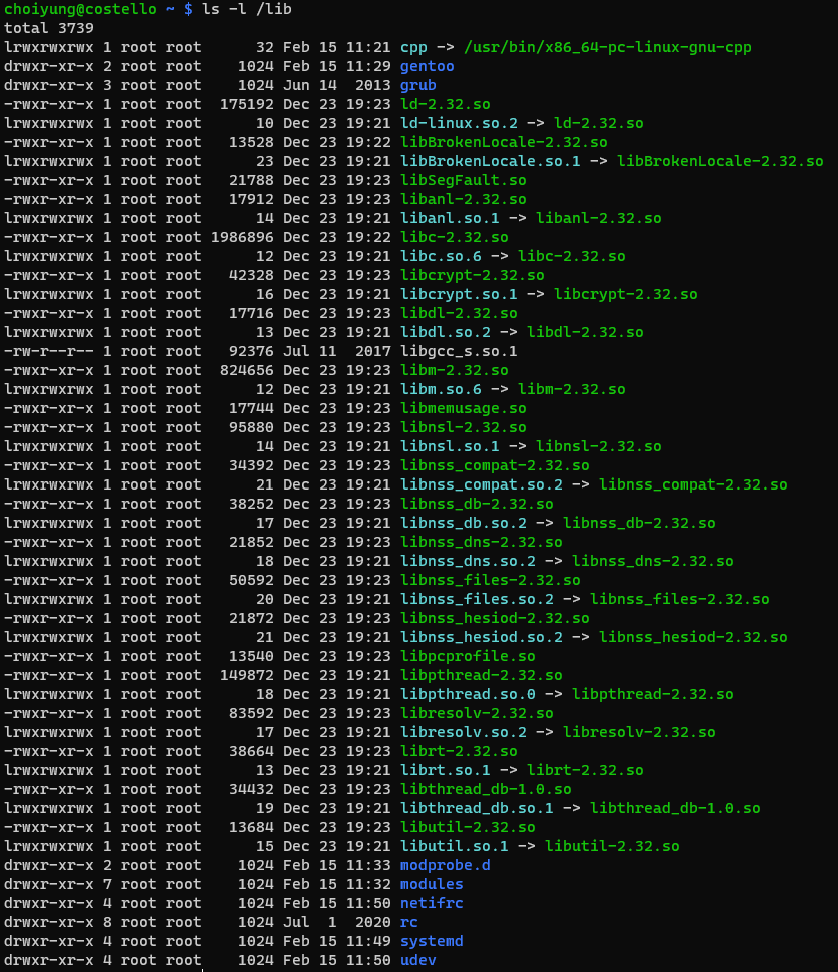
\includegraphics[width=0.75\textwidth]{ECE4310_proj1_part1_1b.png}
\end{figure}

\begin{figure}[H]
  \caption{Output of \texttt{ls -l /var/log}}
  \centering
  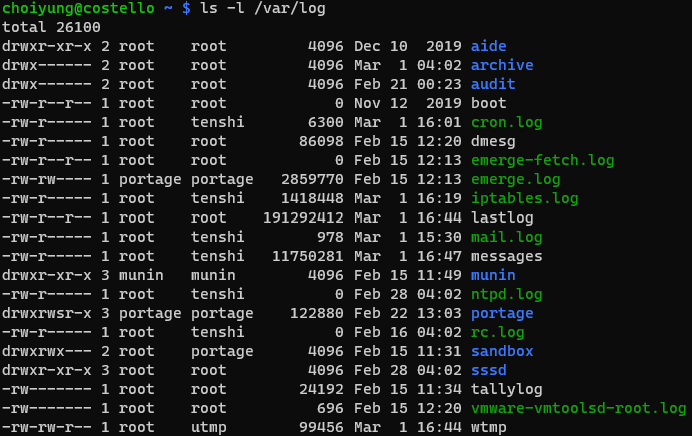
\includegraphics[width=0.75\textwidth]{ECE4310_proj1_part1_1c.png}
\end{figure}

\subsection{\texttt{uname -a}}

\begin{figure}[H]
  \caption{Output of \texttt{uname -a}}
  \centering
  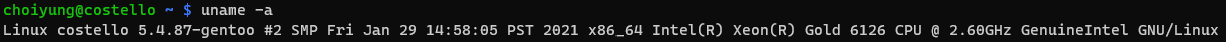
\includegraphics[width=\textwidth]{ECE4310_proj1_part1_2.png}
\end{figure}
It uses 5.4.87-gentoo release of the Linux kernel. It was compiled on Fri Jan 29 14:58:05 PST 2021 for x86\_64 architecture.

\subsection{\texttt{cat /proc/meminfo}}
\begin{figure}[H]
  \caption{Output of \texttt{cat /proc/meminfo}}
  \centering
  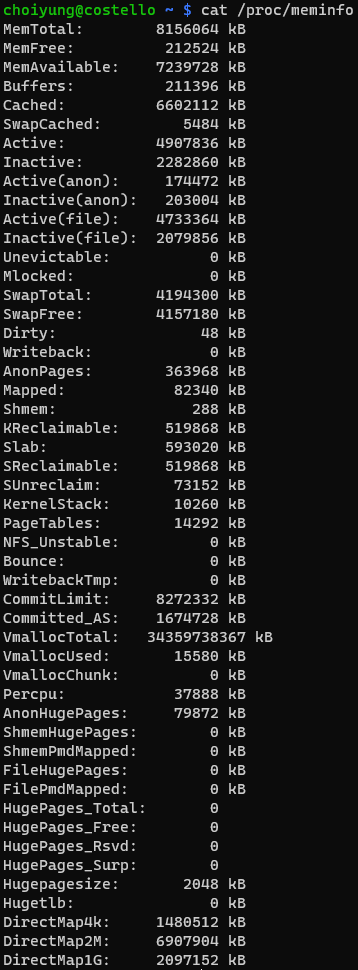
\includegraphics[width=0.35\textwidth]{ECE4310_proj1_part1_3.png}
\end{figure}
212524 MB memory is free and $8156064-212524=7943540$ MB memory is used.
\newpage
\subsection{\texttt{cat /proc/cpuinfo}}
\begin{figure}[H]
  \caption{Output of \texttt{cat /proc/cpuinfo}}
  \centering
  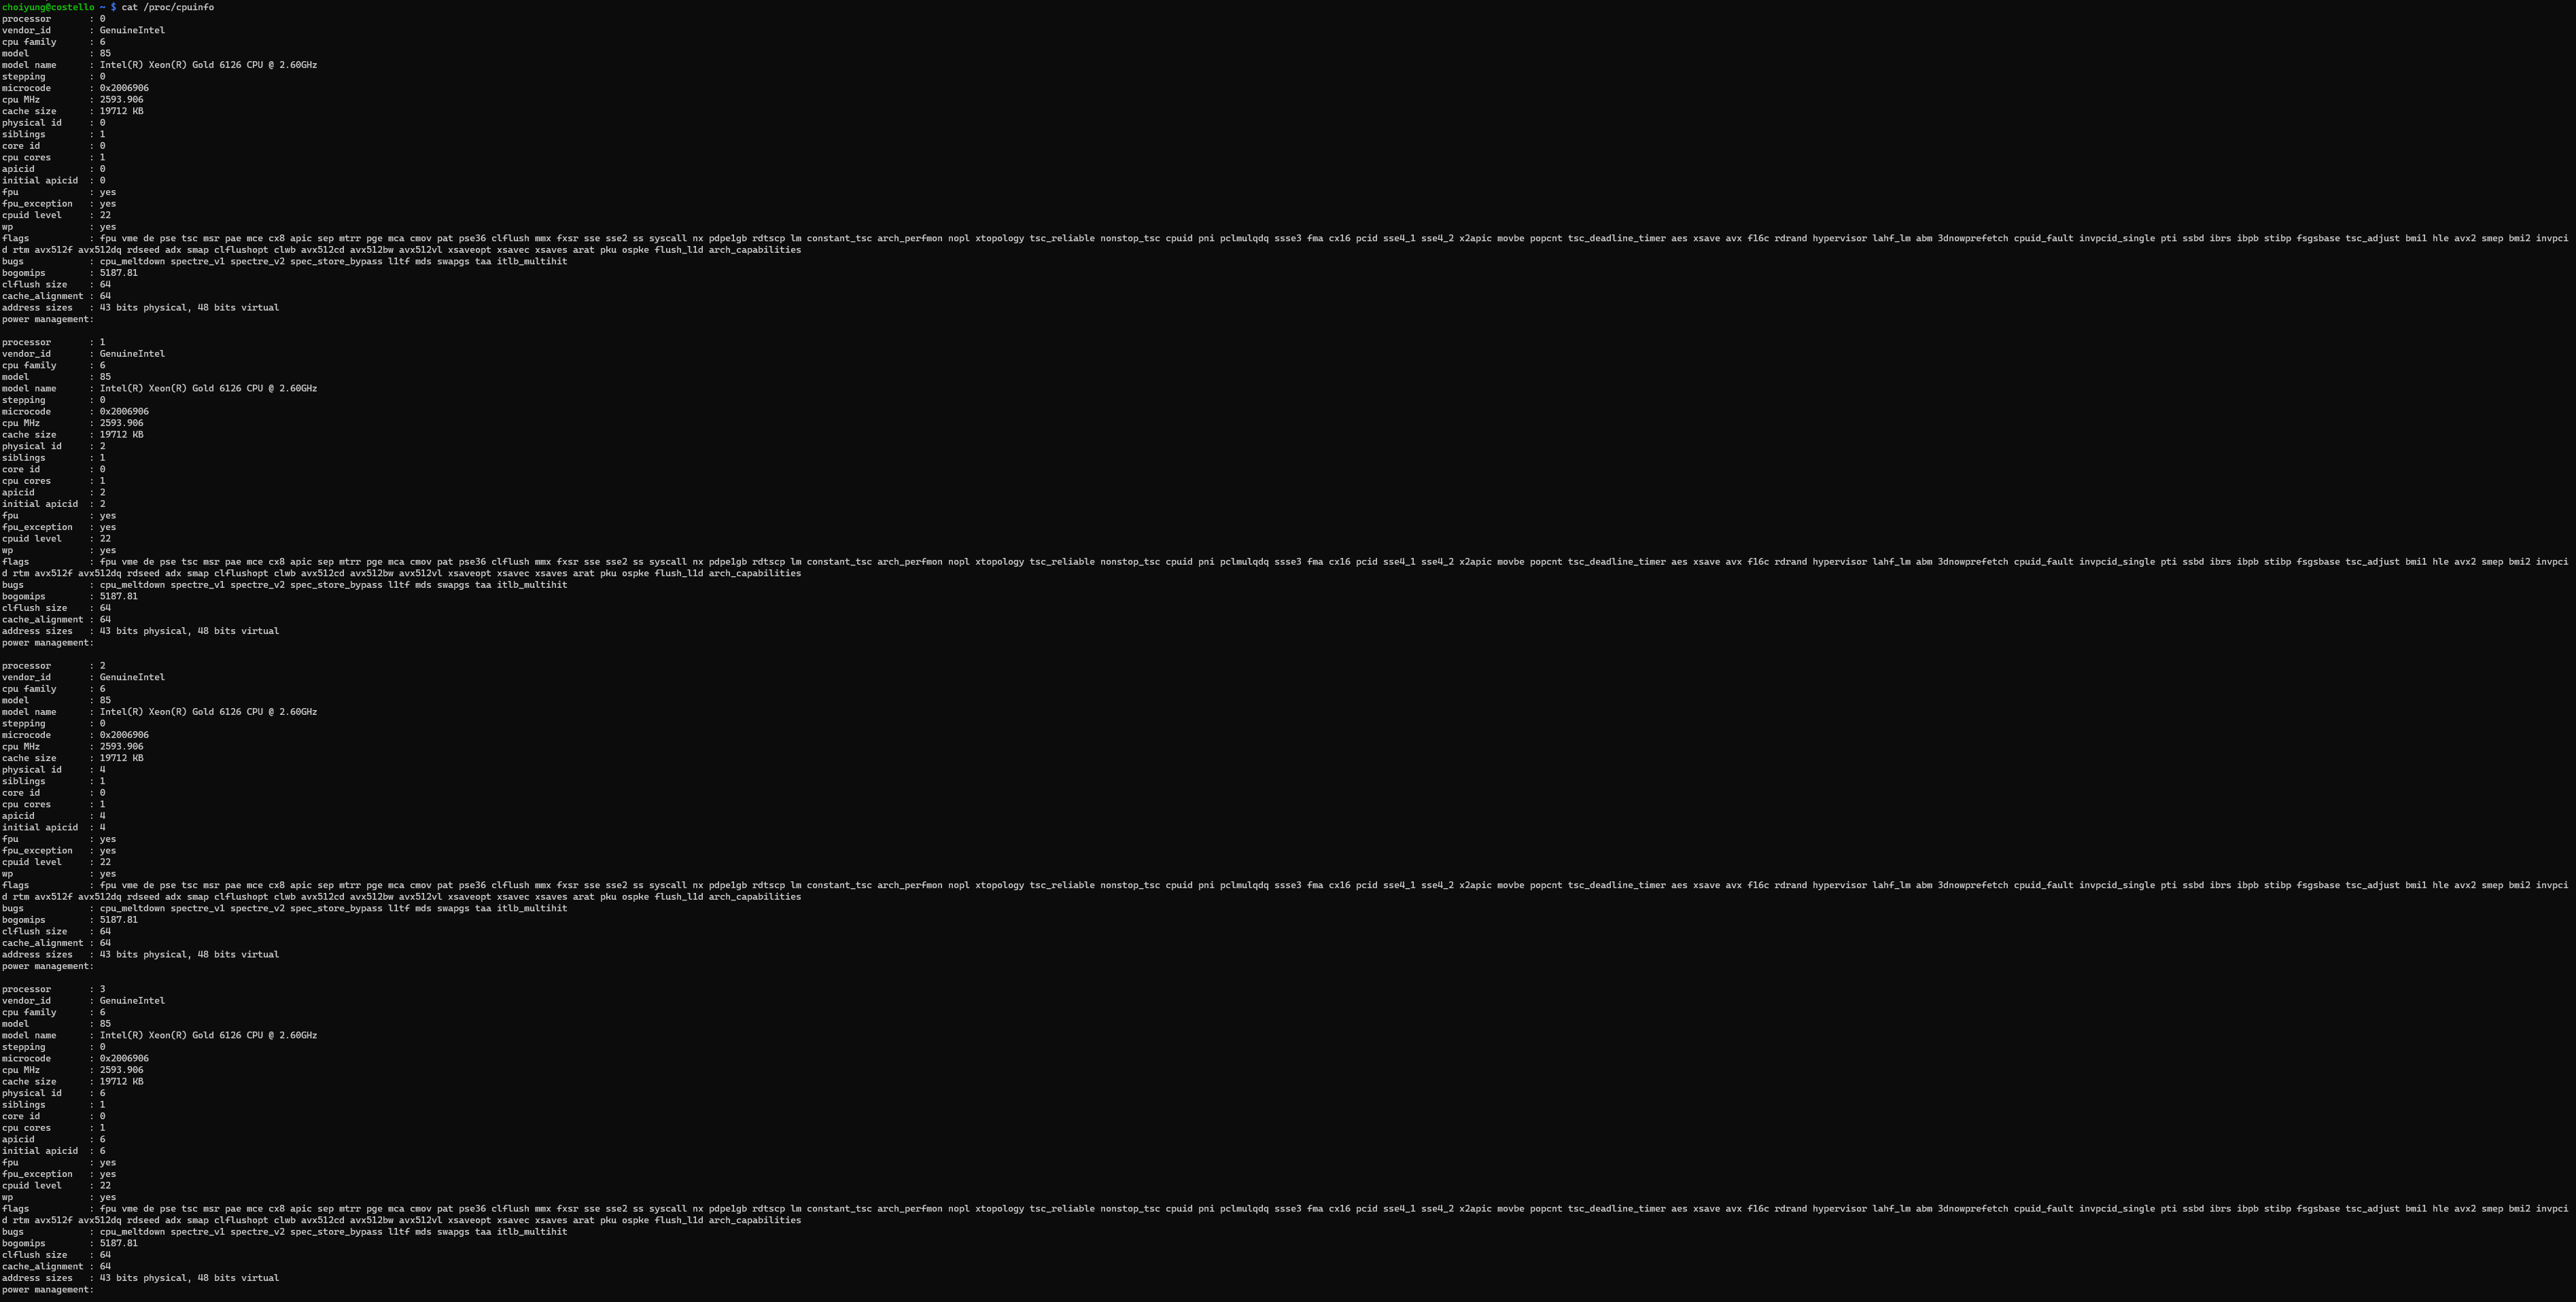
\includegraphics[width=\textwidth]{ECE4310_proj1_part1_4a.png}
\end{figure}
\begin{figure}[H]
  \caption{Output of \texttt{cat /proc/cpuinfo} cont.}
  \centering
  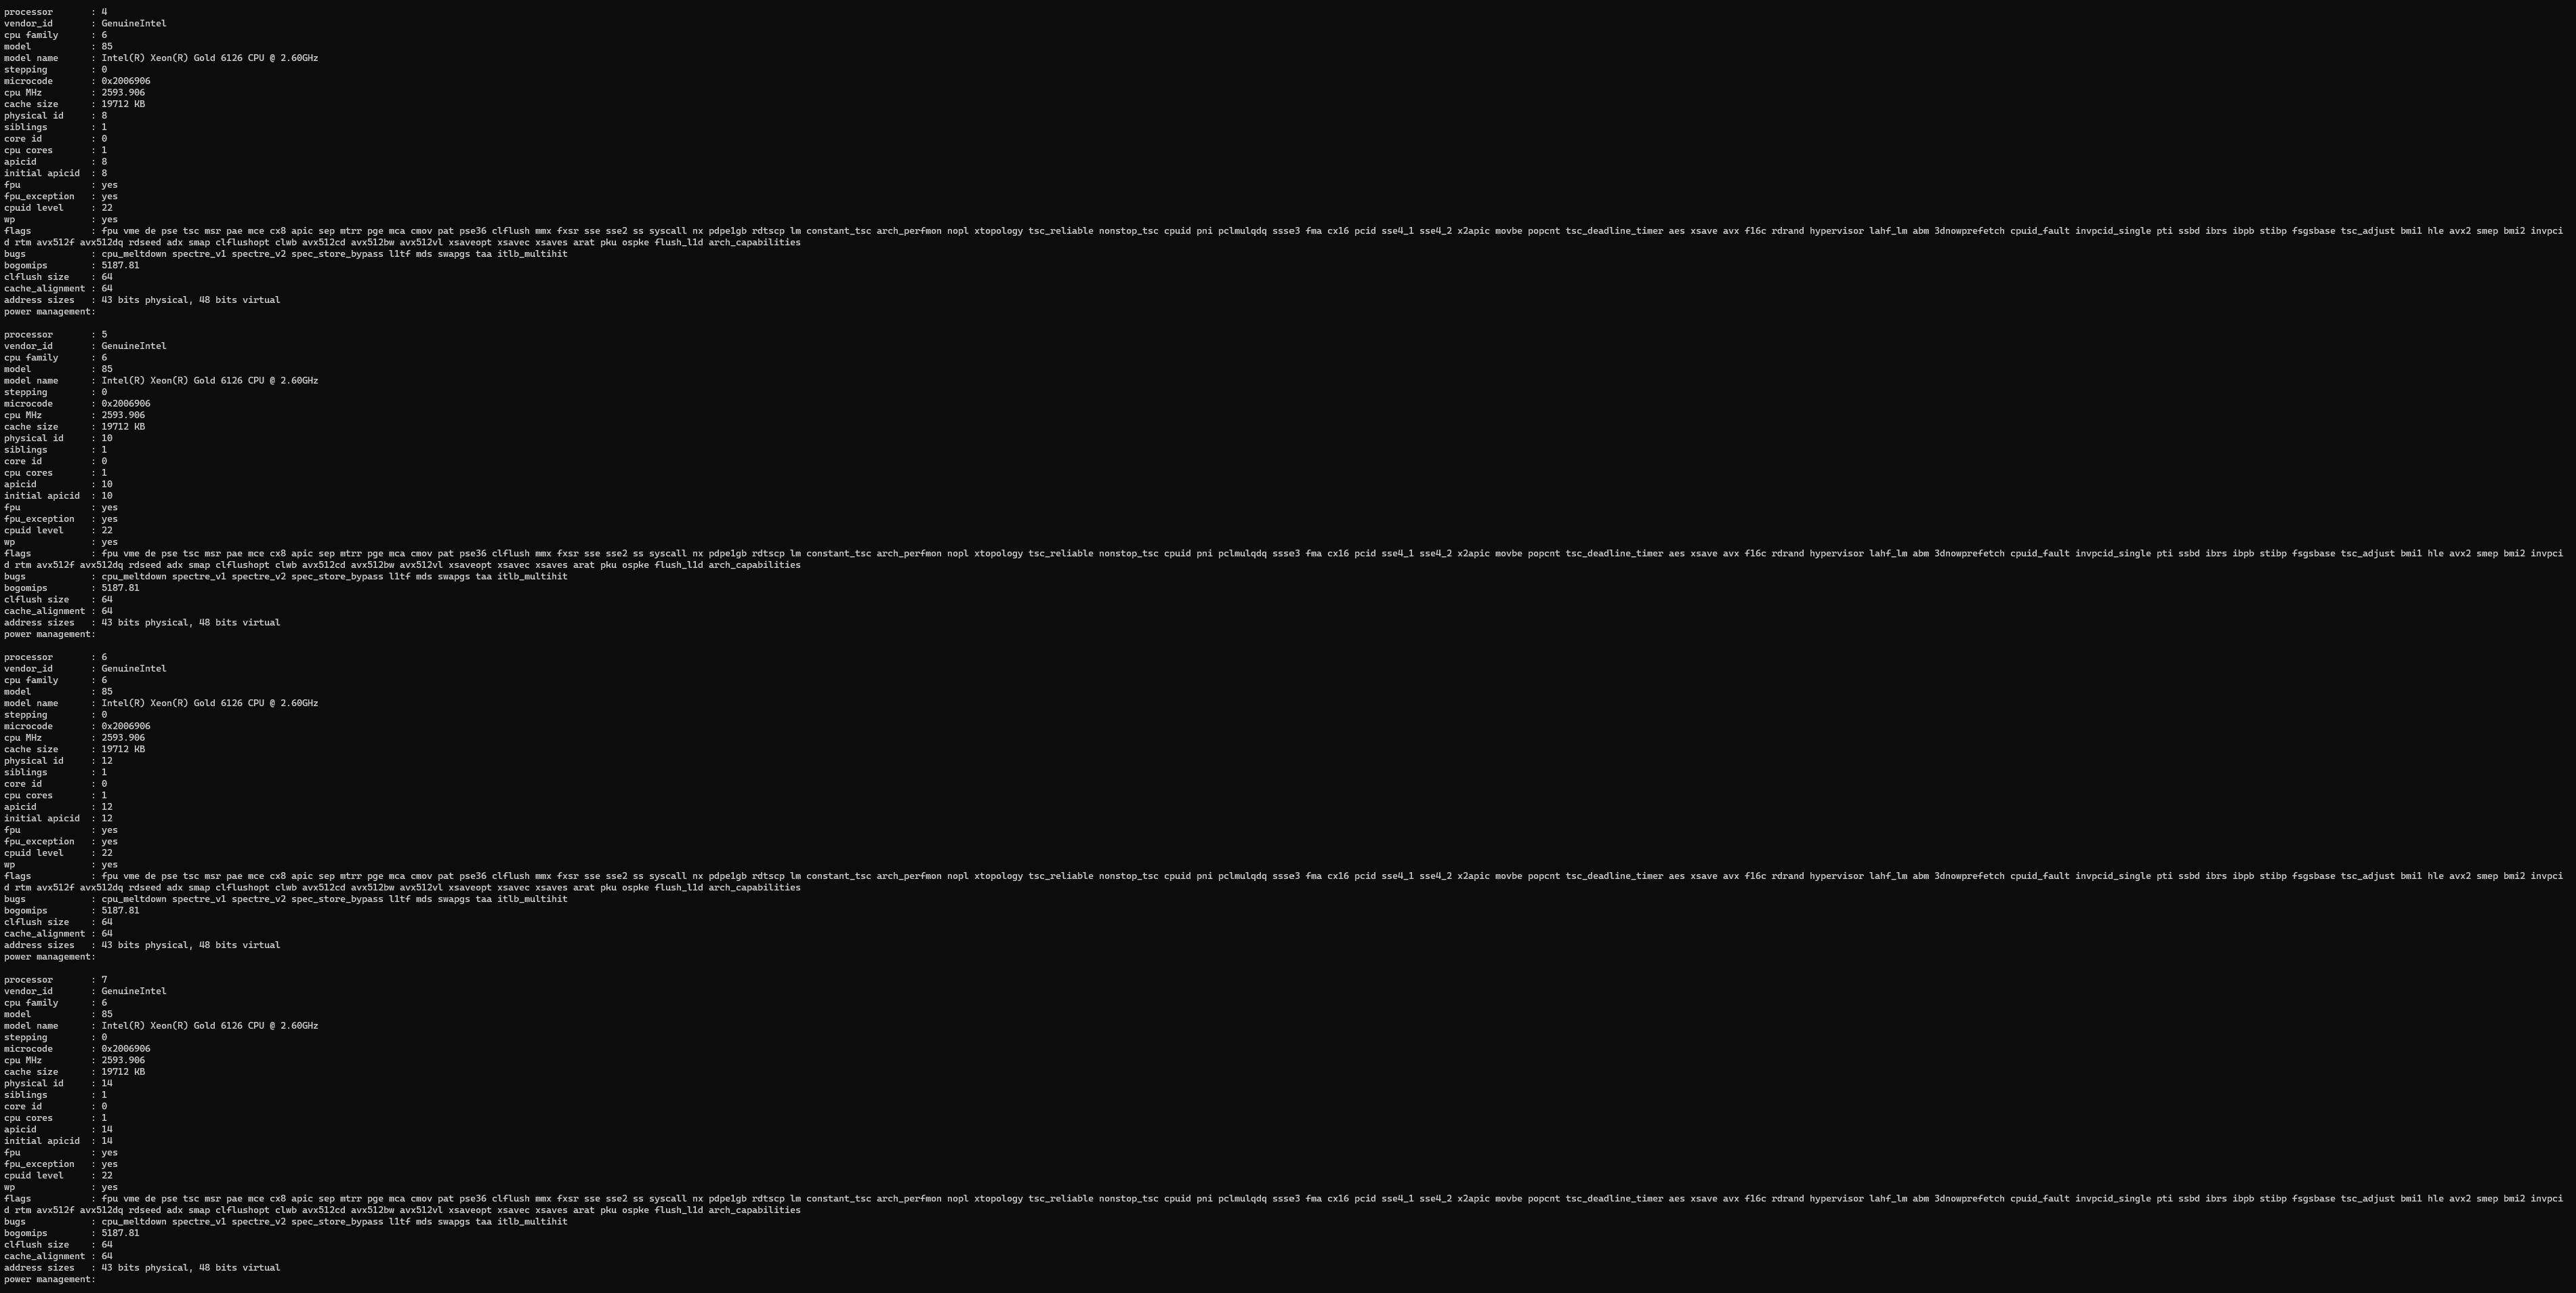
\includegraphics[width=\textwidth]{ECE4310_proj1_part1_4b.png}
\end{figure}

There are a total of 8 CPUs that the operating system see and they are all Intel Xeon Gold 6126.

\subsection{\texttt{nano -w project1-choiyung}}
\begin{figure}[H]
  \caption{Output of \texttt{ls} after \texttt{nano}}
  \centering
  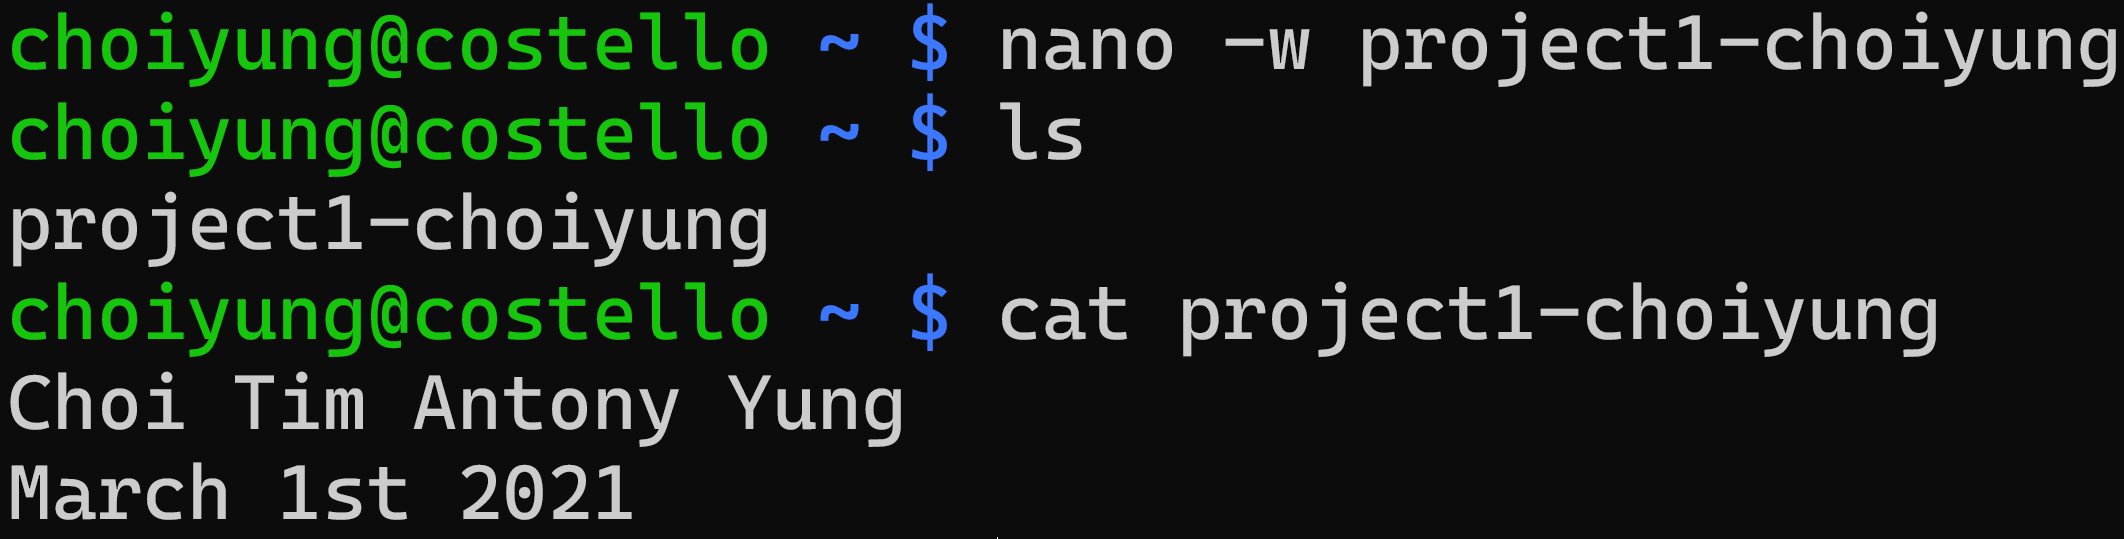
\includegraphics[width=\textwidth]{ECE4310_proj1_part1_5.png}
\end{figure}

\subsection{\texttt{ifconfig eth0}}
\begin{figure}[H]
  \caption{Output of \texttt{ifconfig eth0}}
  \centering
  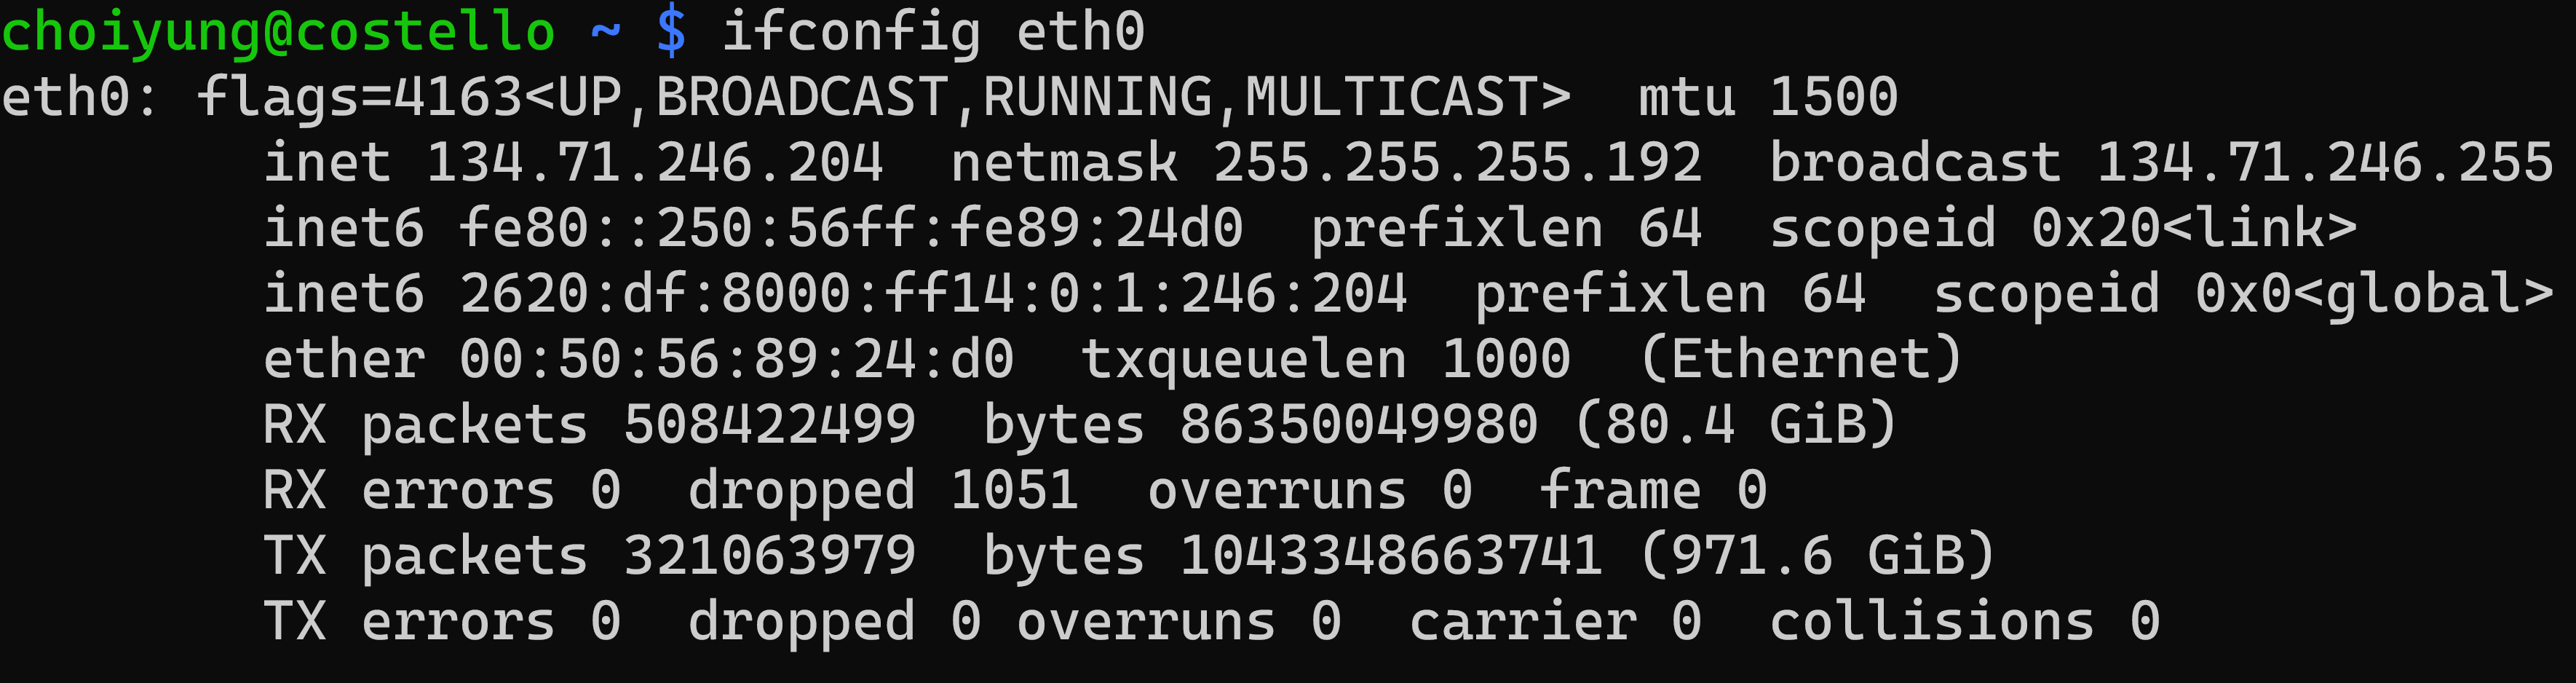
\includegraphics[width=\textwidth]{ECE4310_proj1_part1_6.png}
\end{figure}
IPv4 address is \texttt{134.71.246.204}, IPv6 address is \texttt{2620:df:8000:ff14:0:1:246:204}, MAC address is \texttt{00:50:56:89:24:d0}

\section{\texttt{ps}}
\begin{figure}[H]
  \caption{Output of \texttt{ps -ef}}
  \centering
  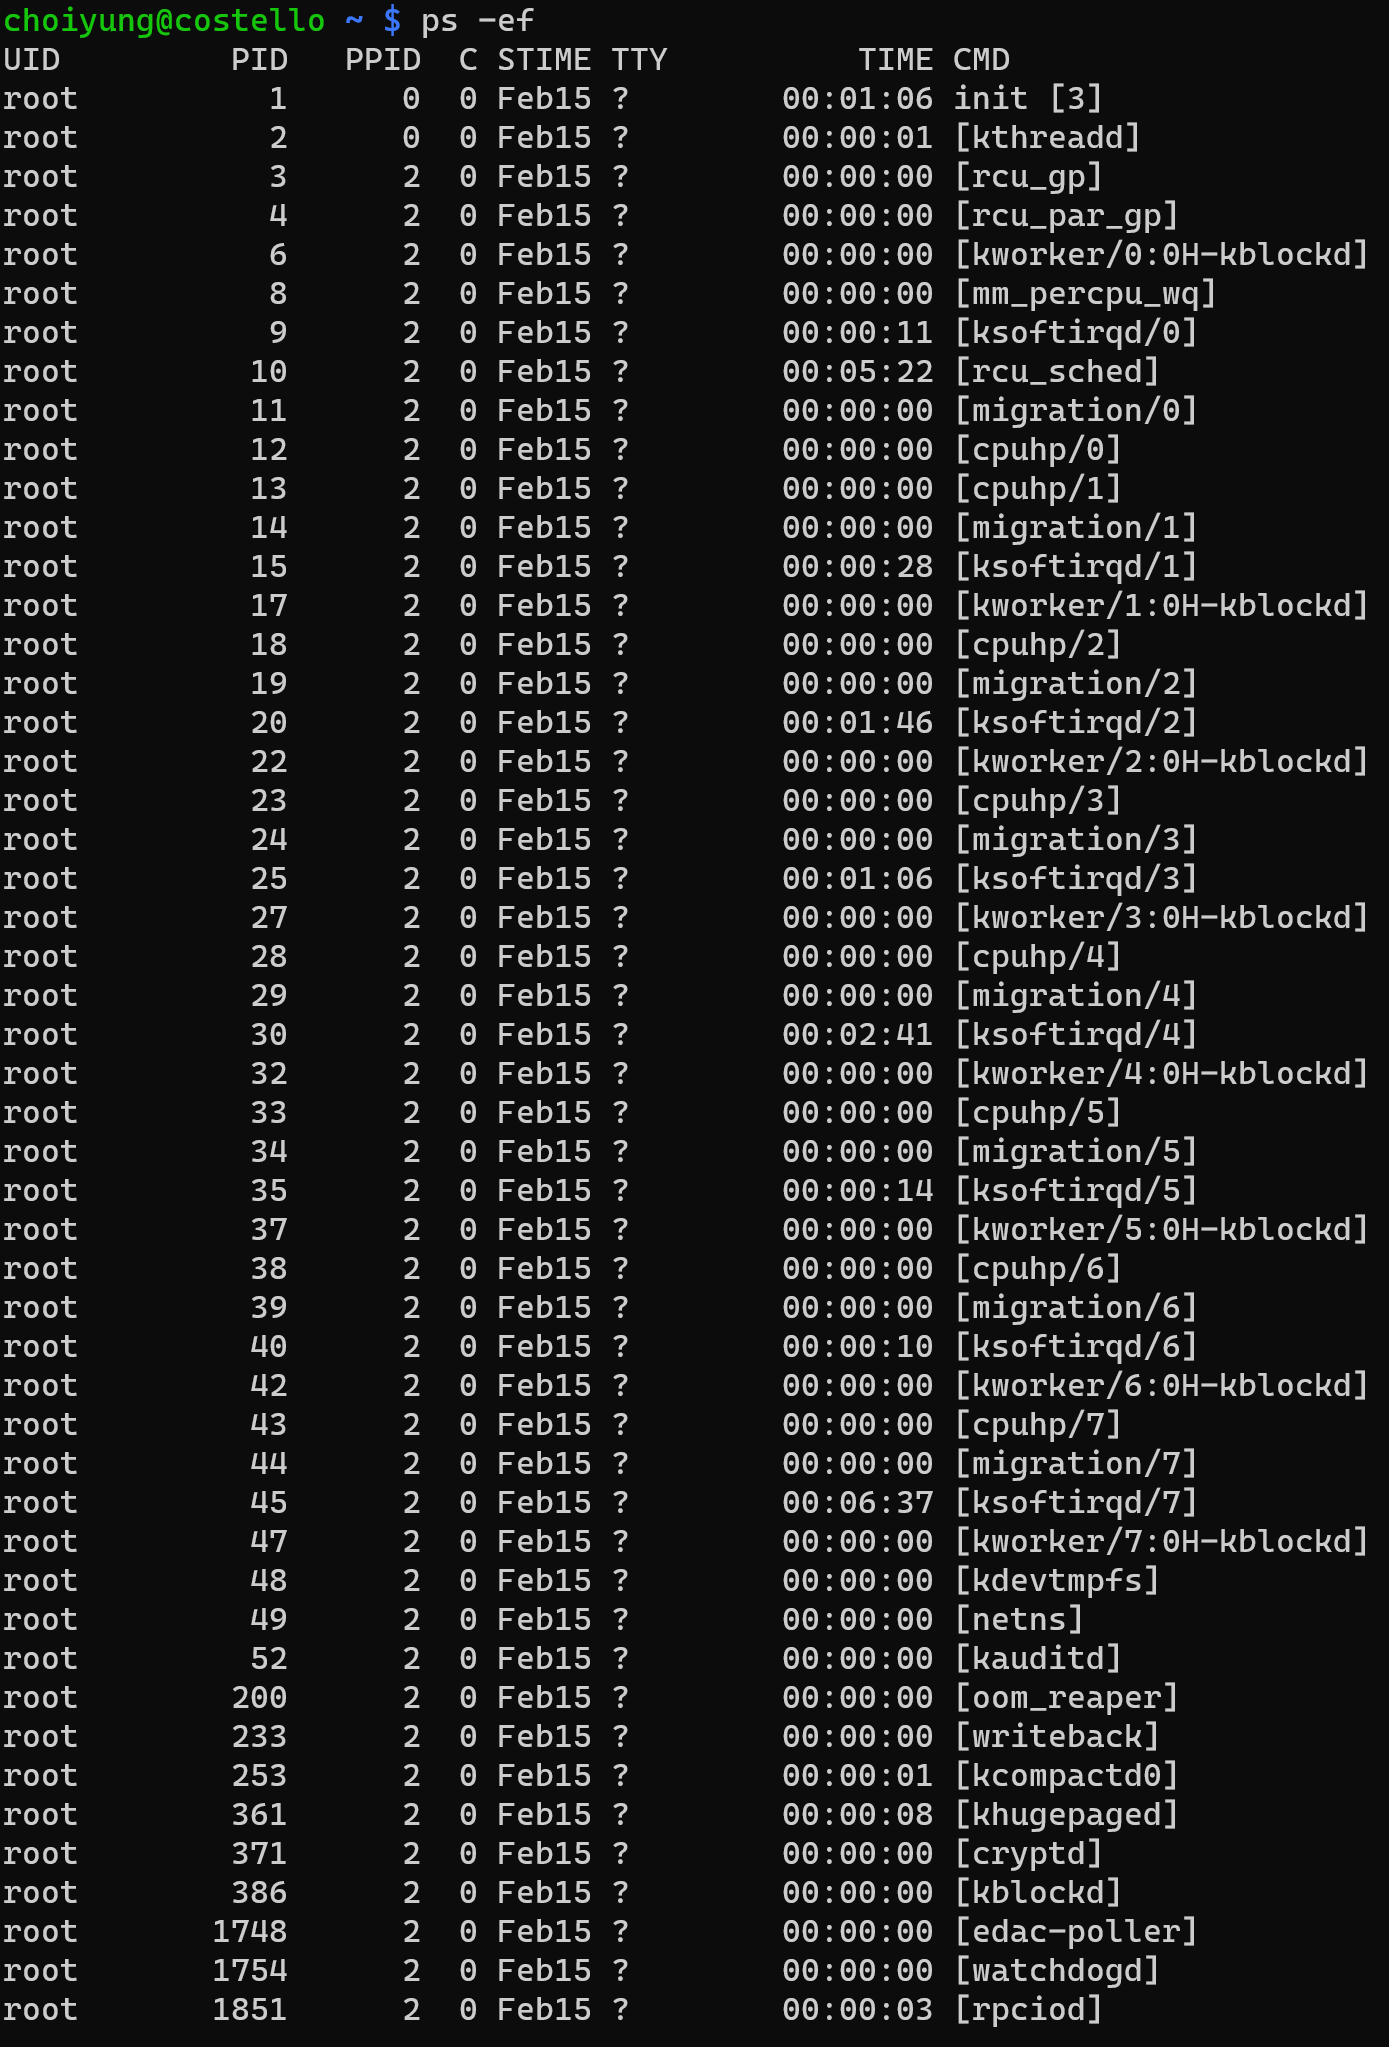
\includegraphics[width=0.5\textwidth]{ECE4310_proj1_part2_ef.png}
\end{figure}
The \texttt{-e} option select all processes and the \texttt{-f} option use full-format listing.
Processes listed with name in square bracket mean the process arguments are unavailable.
\begin{figure}[H]
  \caption{Part of \texttt{man ps}}
  \centering
  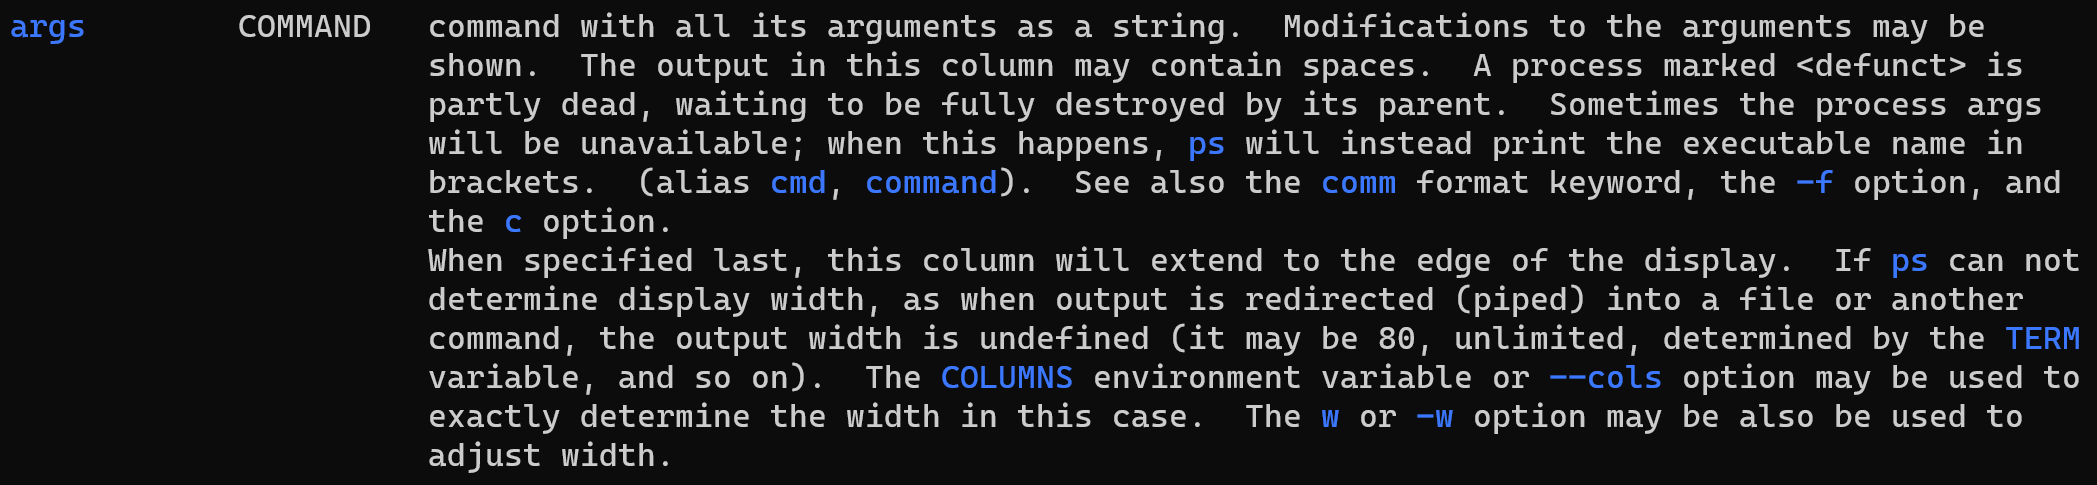
\includegraphics[width=0.75\textwidth]{ECE4310_proj1_part2_bracket.png}
\end{figure}

\newpage
\begin{figure}[H]
  \caption{Output of \texttt{ps -f --ppid 2 --pid 2 --deselect}}
  \centering
  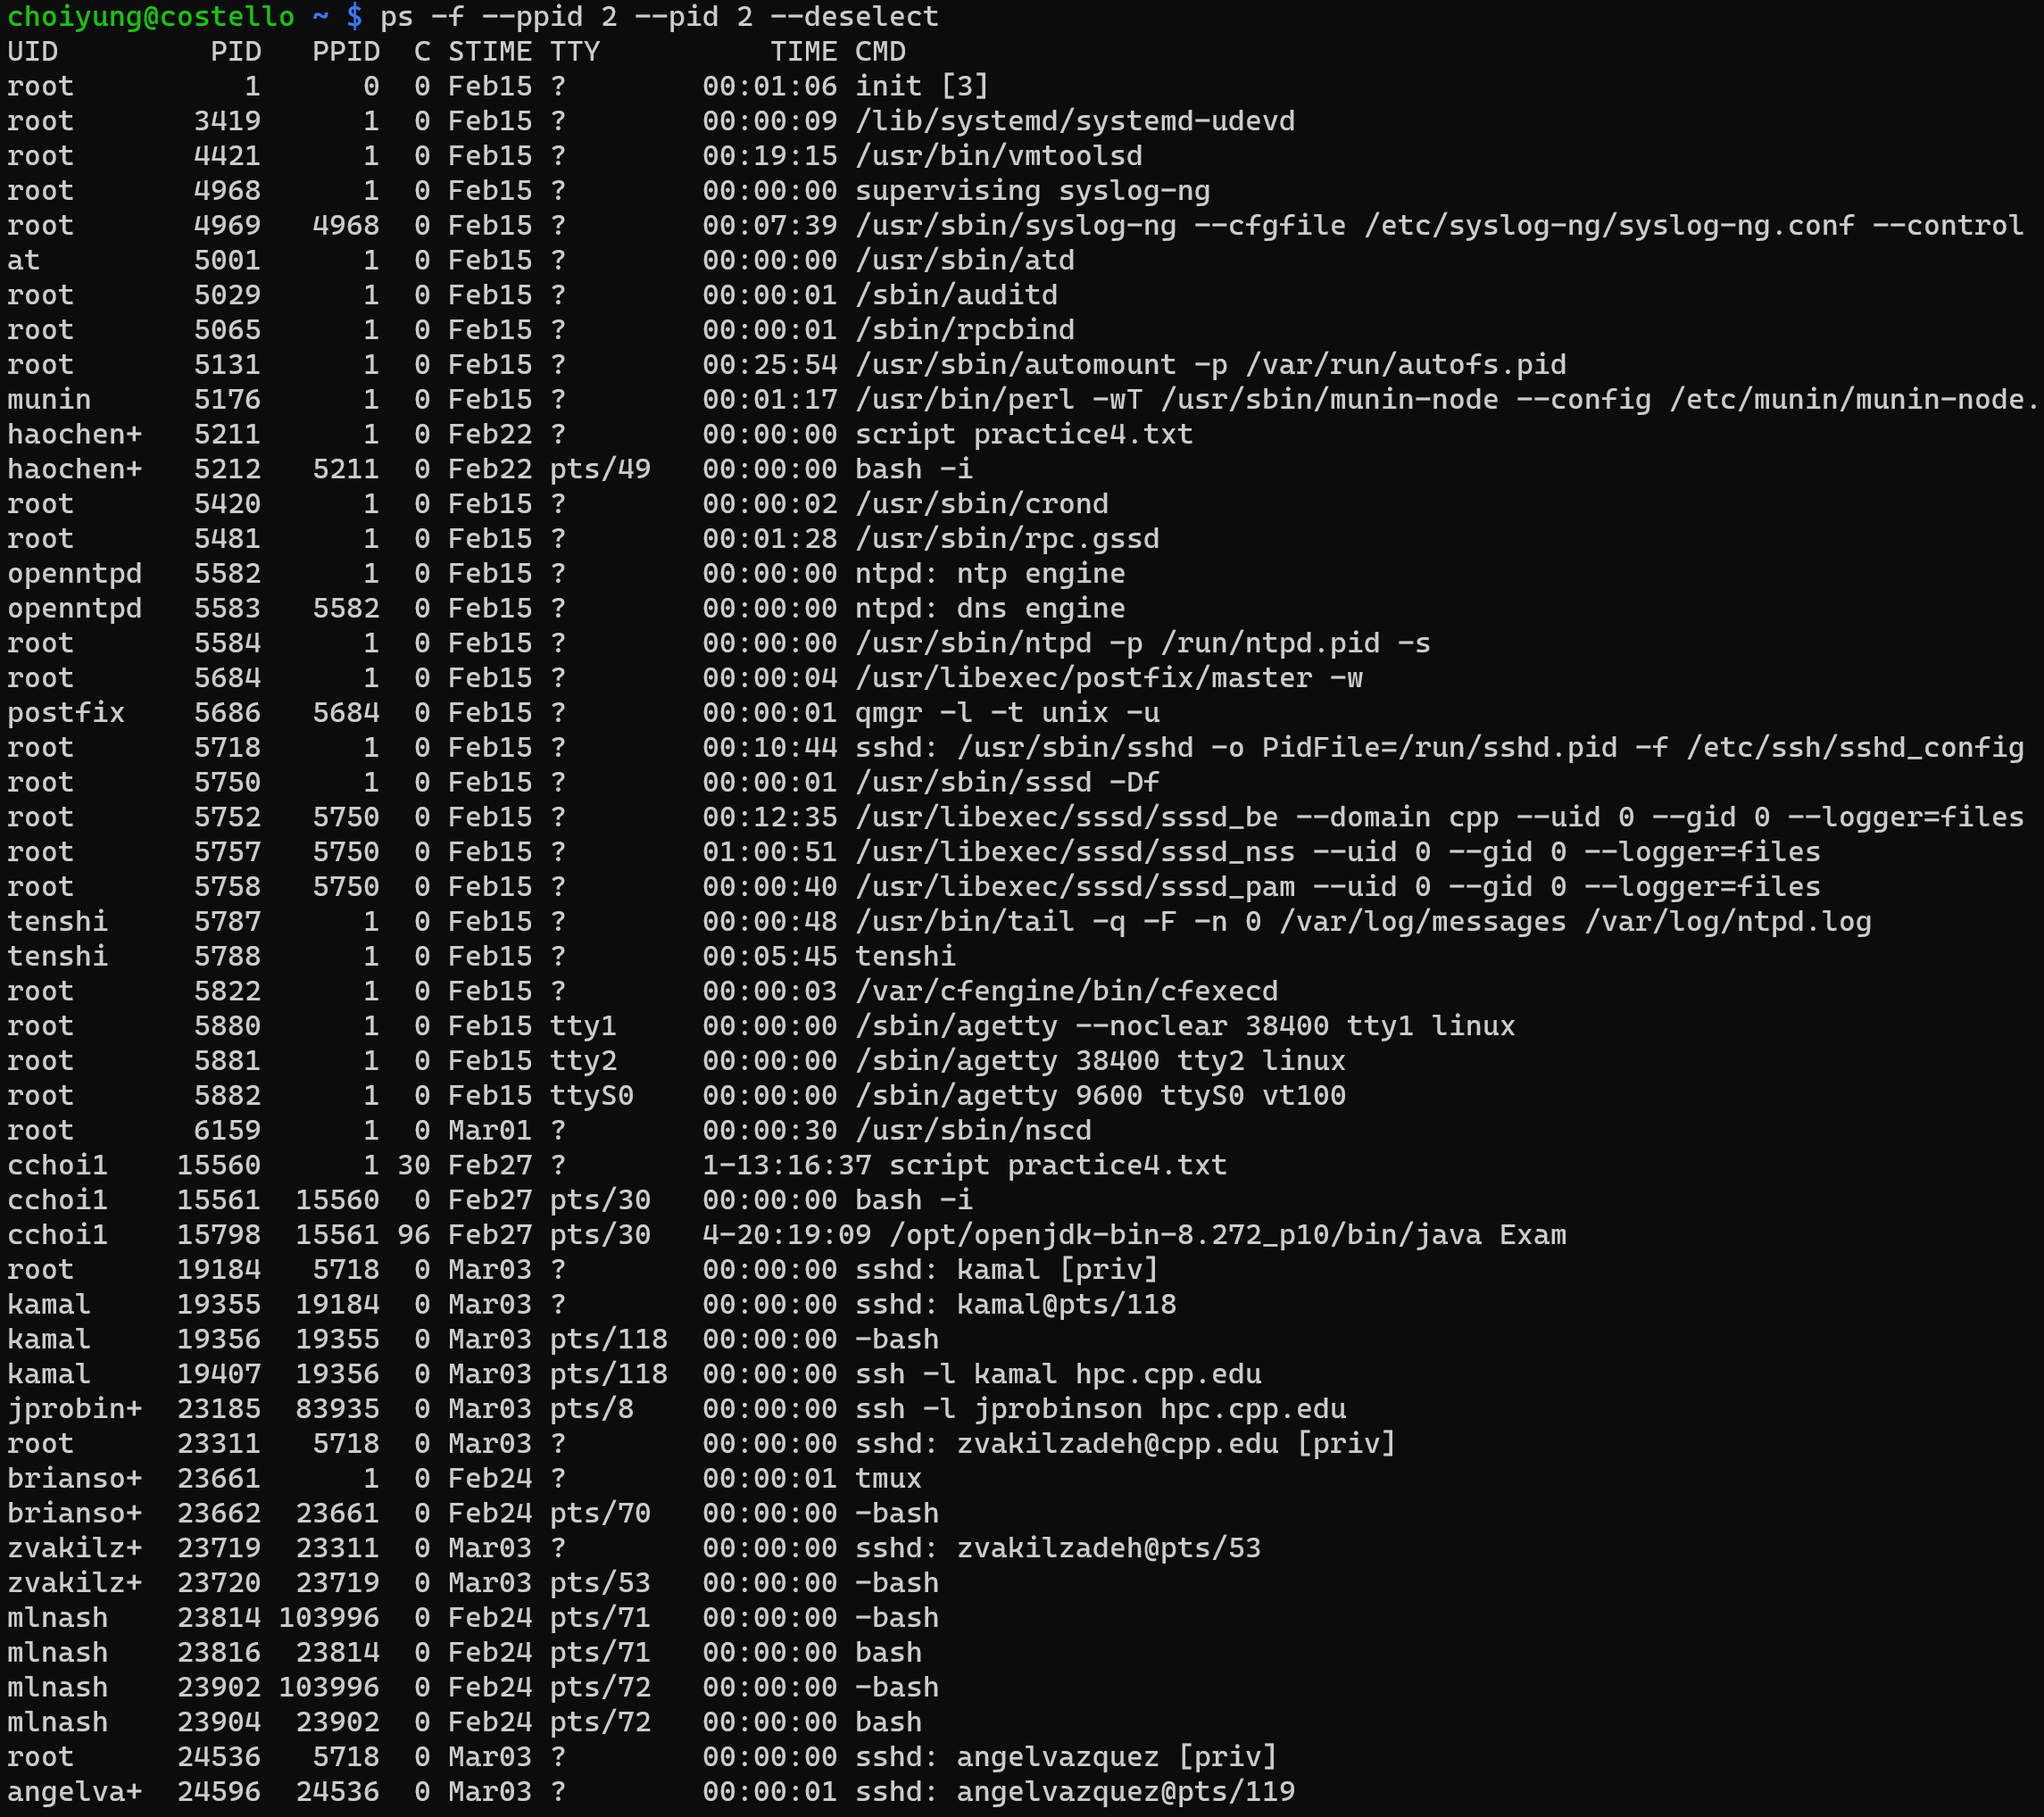
\includegraphics[width=0.5\textwidth]{ECE4310_proj1_part2_deselect.png}
\end{figure}
Kernel threads are spawn by the kernel thread daemon \texttt{kthreadd}, which have \texttt{pid} of \texttt{2}.
\texttt{--ppid 2} option select all child processes of \texttt{kthreadd}, while \texttt{--pid 2} option select \texttt{kthreadd} itself. 
The two options combined will select all kernel threads. \texttt{--deselect} option will then negates the selection which result in all user-space threads selected.
\begin{figure}[H]
  \caption{Output of \texttt{ps -ef | grep choiyung}}
  \centering
  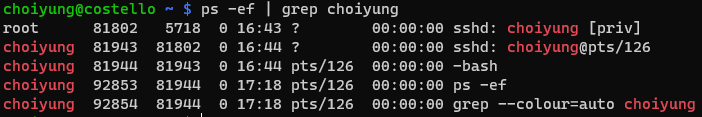
\includegraphics[width=\textwidth]{ECE4310_proj1_part2_grep.png}
\end{figure}
5 processes was associated with my username. Two from the secure shell daemon, one from the bash shell, one from the ps command and one from the grep command. 
\end{document}